\documentclass[conference]{IEEEtran}
\IEEEoverridecommandlockouts
% The preceding line is only needed to identify funding in the first footnote. If that is unneeded, please comment it out.
\usepackage{cite}
\usepackage{amsmath,amssymb,amsfonts}
\usepackage{algorithmic}
\usepackage{graphicx}
\usepackage{textcomp}
\usepackage{xcolor}
\graphicspath{ {./} }
\def\BibTeX{{\rm B\kern-.05em{\sc i\kern-.025em b}\kern-.08em
    T\kern-.1667em\lower.7ex\hbox{E}\kern-.125emX}}
\begin{document}

\title{Toxic issues in Github\\}

\maketitle

\begin{abstract}
Abstract 
\end{abstract}

\begin{IEEEkeywords}
Keywords 
\end{IEEEkeywords}

\section{Introduction}
Introduction
\section{Related Works}
Related works 

\section{Data and Methods}
We designed a classification scheme to identify potentially toxic issues and comments on Github. We used SVM classifiers along with leveraging differences between Software Engineering and English vocabularies to classify issues accurately. We demonstrated that our scheme performs well for both in-sample and out-of-sample testing, and we later used our scheme to analyze trends in Github. 

\subsection{Data}
Our source of data is the June 2019 version of GHTORRENT \cite{b2} , a database of Github issues and comments. The database contained over 80 million issues, some of which were deleted on Github but still available on the database. Each issue had metadata about its origin including creator and creation date, and each comment contained its text and the issue it's associated with. 


To predict toxic issues, we created a training dataset by labeling  comment toxicity, and then labeled issues as toxic if they contained one or more toxic comments. To find examples of toxic comments, we labeled issues that were marked by Github as "too heated." We labeled 179 issues, of which 73 were toxic and 106 were non-toxic. To increase our training size, we labeled 225 random issues on github, all of which were non-toxic. Finally, we used our Active Learning procedure to label 51 more issues, of which 20 were toxic and 31 were non toxic. In the end, our training data set contained 455 issues, with 93 toxic issues, and 362 non-toxic issues. 


For each comment, we kept track of heuristics and external metrics used to score comments. 
\begin{table}[]
	\begin{tabular}{|p{2cm}|p{6cm}|} \hline
		\textbf{Feature} & \textbf{Description}                                                                                        \\ \hline
		Num Emojis       & Number of Emojis                                                                                             \\ \hline
		Num Urls         & Number of URLs                                                                                              \\ \hline
		Length           & Length in Characters                                                                                        \\ \hline
		Stanford Polite  & Using \cite{b8} we give a 0-1 score of politeness, where 0 is the least polite, and 1 is the most polite     \\ \hline
		Perspective      & Using \cite{b7}, we give a 0-1 score of how toxic comments are, where 0 is the least toxic and 1 is the most \\ \hline
		Subjectivity     & Using TextBlob sentiment, get a 0-1 score of subjectivity, where 1 is the most subjective                   \\ \hline
		Polarity         & Using TextBlob sentiment, get a -1-1 score of polarity, where 1 and -1 are the most subjective              \\ \hline
		NLTK Vader       & Using VADER sentiment analyzer \cite{b9}, we find the compound sentiment score                             \\ \hline
		TF IDF           & Use TF IDF word frequencies                                                                                 \\ \hline
		Anger            & Number of words from Anger Lexicon \cite{b10}                                                               \\ \hline
		Negative         & Number of words from Negative Lexicon \cite{b10} \\  \hline                                                           
	\end{tabular}
\end{table}

\subsection{Model} 

To label a set of issues, we first filtered out non-English or epmty issues. We used an SVM to classify comments as toxic or non-toxic because SVMs are often used for text classification purposes \cite{b11} and because SVMs outperformed other classifiers we tried.

We used two additional techniques along with our classifier to improve performance. 

\textbf{Anger Direction} - We filtered out self directed toxicity to avoid falsely classifying phrases such as "I'm so stupid." These phrases typically indicate self loathing rather than toxicity, and would not contribute to the toxicity of a discussion. We used a classifier from \cite{b3}, that classifies the direction of anger as either self, other person or object, and remove all comments where the anger direction is self.  

\textbf{Software Engineering Words} - Words in software engineering could have different connotations from words in English, such as differences in the meaning of the word "bug." To alleviate this issue, we identified words that are significantly more frequent in software engineering using Log Odds with Dirichlet prior \cite{b12}. Our software engineering corpus came from a random sample of 10K github issues, and our regular English corpus came from the Python library wordfreq \cite{b13} We removed each of these words, re-compute the features for the comment, and re-classify using the new features (We don't do this yet, but we should do this).  


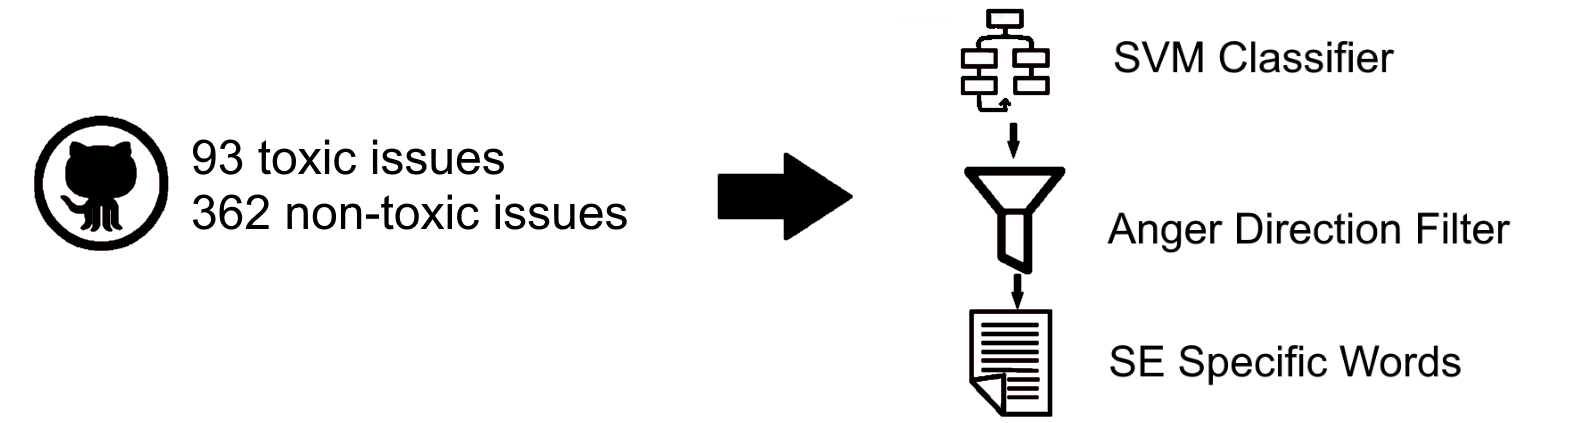
\includegraphics[width=6cm]{pipeline.png}


\subsection{Internal Validation} 
We used 10-fold nested cross validation to tune our hyperparameters and evaluate our model \cite{b14}. Because of the imbalance in the training dataset, for each train-test split, we adjusted the class weights, with a ratio $r$ between non-toxic and toxic examples, where $r$ is a hyperparameter. We tried using ADASYN and SMOTE, but neither provided any significant improvement. We grid searched over hyperparameters $\gamma=\{1,2,2.5,3\}$, $C=\{0.01,0.05,0.1,0.5,1,10\}$ and $r=\{1,1.5,1.75,2,2.25\}$ in our train-validation split. We iteratively added features to find the best feature combination.

To quantify model performance, we used $F_{0.5}$ score, because of the imbalance of our dataset, and because we wanted a precise classifier when run over larger datasets. 

\subsection{Internal Validation Results} 

Our model performed best when using Politeness, Perspective and filtering out Anger Direction and Software Engineering Words, at $\gamma=2$, $C=0.05$, and $r=2$. We obtained a score of $f_{0.5}=0.736$, with a precision of $0.91$ and recall of $0.42$. We demonstrated that the addition of new features does not significantly improve model performance. Additionally, the removal of features from our model significantly detracted from model performance. 

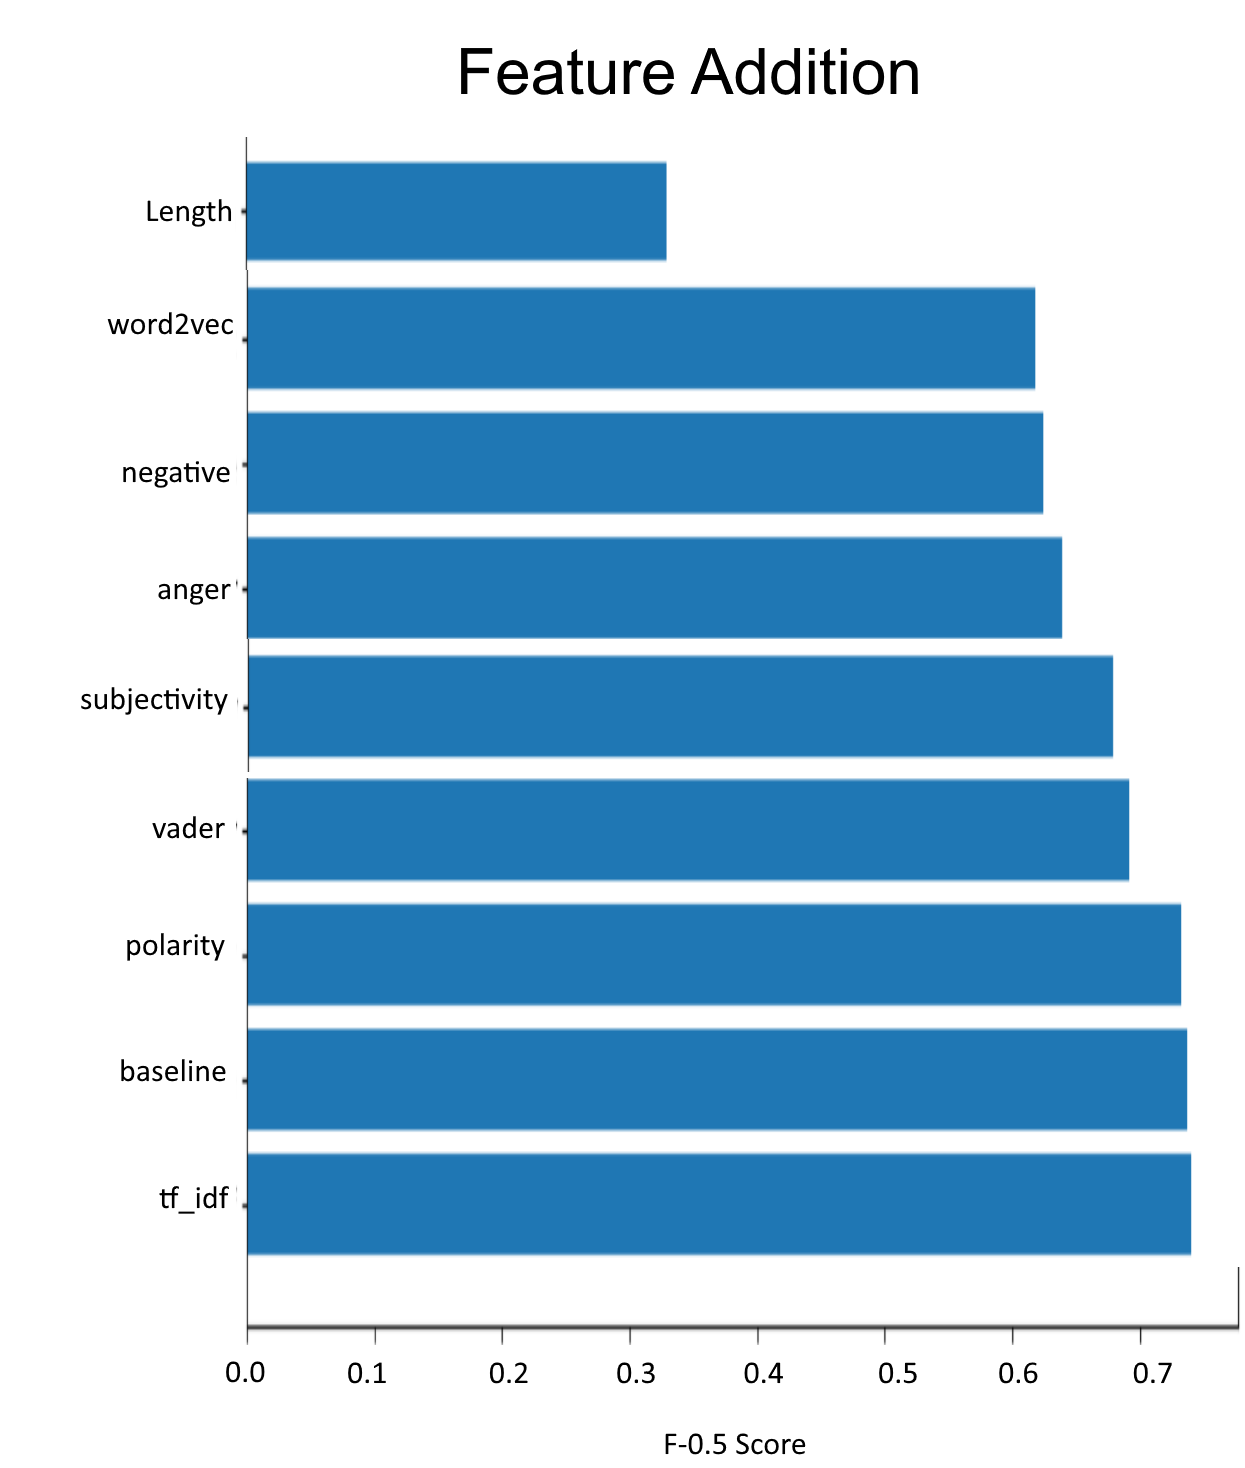
\includegraphics[width=6cm]{feature.png}

\subsection{External Validation} 

We performed external validation by selecting, at random 100K issues from Github. We filtered out non-English and non-Empty issues, and classified them. We selected 100 issues that were classified as toxic, and classified them by hand in an effort to demonstrate the precision of our model. 

\subsection{External Validation Results} 

\section{Experiments} 
\subsection{Toxicity over time} 
We explored whether the percentage of toxic comments on Github has increased over time. Because of the infeasibility of classifying every issue on Github, we selected all the issues from each second monday from January 2012-December 2018. We selected the date so to account for confounding factors such as the day of the week, or the time of the month. (CITATION?)

We saw that the number of issues has increased significantly over that time span.
 
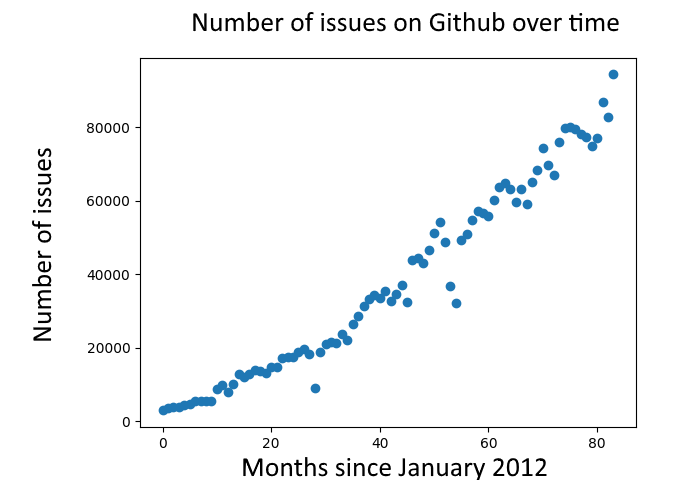
\includegraphics[width=10cm]{issues_per_month.png}

\subsection{Corporate vs. Non-Corporate} 
We explored whether corporate projects are more or less toxic than non-corporate projects. To find corporate issues, we found the top 1000 projects run by some organization or company, removed non-English projects, sorted by number of contributors from that organization, and took the top 100 issues. None of the top 100 projects were from academic or university sources. We selected all the issues from each of the top 100 projects. 

To find non-corporate projects, we sorted the most popular projects by the number of stars, and selected the top 100 projects that were not run by some company or organization. Again, none of the top 100 were from academic sources. We again selected all the issues from each of the top 100 projects. 

\subsection{Community differences} 
Previous work suggests that there exists cultural differences between communities \cite{b15}. We explored toxicity differences between issues from projects in three popular languages: Python, Java and Javascript \cite{b16}. We selected 1000 issues at random from each of the three languages, and classify them as toxic or non-toxic. 

\section{Results and Discussion}
Results and Discussion

\section{Threats to Validity}
Threats to Validity

\section{Conclusion}
Conclusion


\begin{thebibliography}{00}
\bibitem{b1} Cohen, Jacob. Statistical power analysis for the behavioral sciences. Routledge, 2013.
\bibitem{b2} Georgios Gousios: The GHTorrent dataset and tool suite. MSR 2013: 233-236
\bibitem{b3} Gachechiladze, Daviti, et al. "Anger and its direction in collaborative software development." 2017 IEEE/ACM 39th International Conference on Software Engineering: New Ideas and Emerging Technologies Results Track (ICSE-NIER). IEEE, 2017.
\bibitem{b4} Scott, Mike, and Christopher Tribble. Textual patterns: Key words and corpus analysis in language education. Vol. 22. John Benjamins Publishing, 2006.
\bibitem{b5} Bonett, Douglas G. "Transforming odds ratios into correlations for meta-analytic research." (2007): 254.
\bibitem{b6} Görnitz, Nico, et al. "Toward supervised anomaly detection." Journal of Artificial Intelligence Research 46 (2013): 235-262. 
\bibitem{b7}  “https://www.perspectiveapi.com/,”
\bibitem{b8} Danescu-Niculescu-Mizil, Cristian, et al. "A computational approach to politeness with application to social factors." arXiv preprint arXiv:1306.6078 (2013).
\bibitem{b9} Hutto, Clayton J., and Eric Gilbert. "Vader: A parsimonious rule-based model for sentiment analysis of social media text." Eighth international AAAI conference on weblogs and social media. 2014.
\bibitem{b10} Zhang, Justine, et al. "Conversations gone awry: Detecting early signs of conversational failure." arXiv preprint arXiv:1805.05345 (2018).
\bibitem{b11} Joachims, Thorsten. "Text categorization with support vector machines: Learning with many relevant features." European conference on machine learning. Springer, Berlin, Heidelberg, 1998.
\bibitem{b12} Monroe, B., Colaresi, M.,\& Quinn, K. (n.d.). Fightin' Words: Lexical Feature Selection and Evaluation for Identifying the Content of Political Conflict. Political Analysis, 16(4), 372-403. doi:10.1093/pan/mpn018
\bibitem{b13} Speer, Robert, et al. "wordfreq: v1. 5.1." (2016).
\bibitem{b14} Fearn, T. (2010). Double Cross-Validation. NIR News, 21(5), 14–15. https://doi.org/10.1255/nirn.1194
\bibitem{b15} Bogart, Christopher, et al. "How to break an API: cost negotiation and community values in three software ecosystems." Proceedings of the 2016 24th ACM SIGSOFT International Symposium on Foundations of Software Engineering. ACM, 2016
\bibitem{b16} Mearian, Lucas. "The state of the octoverse 2018. Computerworldhttps."
\bibitem{b17} https://datastudio.google.com/u/0/reporting/0ByGAKP3QmCjLU1JzUGtJdTlNOG8/page/Q3DM

\end{thebibliography}


\end{document}
